\section{像差工程实践}

\subsection{像差的本质与分类}

\englishtitle{Aberrations in Machine Vision}
\begin{frame}{像差:光学设计的固有属性}
    \begin{columns}[T]
        \begin{column}{.60\textwidth}
            \begin{block}{核心观点}
                光学像差不是由制造缺陷(物理、光学或机械)引起的，而是\alert{透镜设计本身固有的}——源于衍射、折射和光的波动性。因此，不存在"完美"镜头。
            \end{block}

            \bigbreak
            像差最终影响:
            \begin{itemize}
                \item \alert{MTF}(调制传递函数)
                \item \alert{光斑尺寸}(Spot Size)
                \item \alert{远心度}(Telecentricity)
                \item \alert{景深}(Depth of Field)
            \end{itemize}
        \end{column}
        \hfill
        \begin{column}{.40\textwidth}
            \begin{figure}
                \centering
                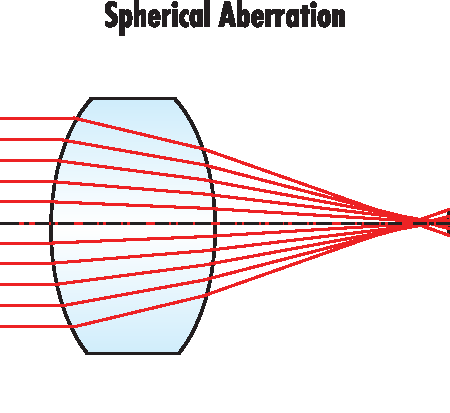
\includegraphics[width=0.95\textwidth]{Figure/Edmund/aberrations-1v2.pdf}
                \caption{球差示意:边缘光线折射更强，焦点更近}
                \label{fig:edmund_spherical_intro}
            \end{figure}
        \end{column}
    \end{columns}

    \alert{关键理解:}像差理论虽然抽象复杂，但理解像差如何影响性能，对应用的成功至关重要。
\end{frame}

\englishtitle{Four Fundamental Aberration Types}
\begin{frame}{四类基本像差概述}
    虽然像差理论体系庞大，但掌握以下四类基本概念即可入门理解:

    \begin{table}
        \centering
        \small
        \begin{tabular}{p{2.5cm}|p{3.5cm}|p{4.5cm}}
            \toprule
            \textbf{像差类型} & \textbf{主要影响因素} & \textbf{对机器视觉的影响} \\
            \midrule
            \alert{球差} & 孔径大小、入射角 & 大光圈镜头成像模糊，需缩小光圈或增加镜片 \\
            \alert{像散} & 视场角、离轴不对称 & 不同方向分辨率不同，子午/弧矢焦点分离 \\
            \alert{场曲} & 佩兹伐和 $\sum\phi_i/n_i$ & 像面弯曲，需负光焦度元件校正 \\
            \alert{色差} & 波长、玻璃色散 & 不同颜色焦点不同，需消色差设计 \\
            \bottomrule
        \end{tabular}
        \caption{Edmund Optics 归纳的四类基本像差}
        \label{tab:four_aberration_types}
    \end{table}

    \alert{注意:}Edmund Optics 将像散和彗差合并讨论("astigmatic aberration")，因其在实际机器视觉镜头中通常共同出现。
\end{frame}

\subsection{球差与像散:孔径与视场的角力}

\englishtitle{Spherical Aberration — Aperture-Dependent Blur}
\begin{frame}{球差:孔径依赖性的模糊}
    \begin{columns}[T]
        \begin{column}{.40\textwidth}
            \begin{figure}
                \centering
                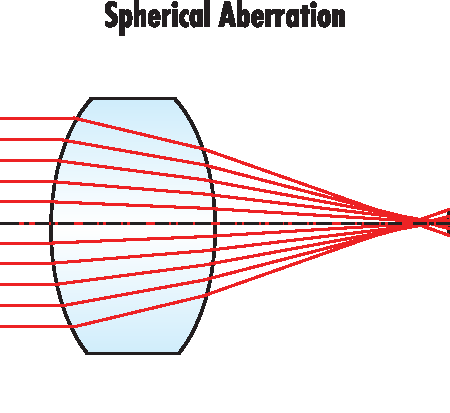
\includegraphics[width=\textwidth]{Figure/Edmund/aberrations-1v2.pdf}
                \caption{球差:边缘光线因入射角大而折射更强}
                \label{fig:edmund_spherical}
            \end{figure}
        \end{column}
        \hfill
        \begin{column}{.60\textwidth}
            \textbf{物理机制:}
            \begin{itemize}
                \item 光线在透镜表面的\alert{入射角}越大，折射越强
                \item 平行光线越靠近透镜边缘，入射角越大
                \item 边缘光线焦点 $\neq$ 近轴光线焦点
            \end{itemize}

            \bigbreak
            \textbf{工程事实:}
            \begin{itemize}
                \item 大孔径(小 $f/\#$)镜头\alert{更容易}受球差影响
                \item 缩小光圈可改善，但\alert{衍射效应}最终会成为限制
                \item 使用高折射率玻璃或增加镜片可校正——但会增加\alert{体积、重量和成本}
            \end{itemize}
        \end{column}
    \end{columns}
\end{frame}

\englishtitle{Spherical Aberration — Correction Tradeoffs}
\begin{frame}{球差校正的工程权衡}
    \begin{columns}[T]
        \begin{column}{.52\textwidth}
            \textbf{校正策略与代价:}

            \begin{enumerate}
                \item \alert{缩小光圈(增大 $f/\#$)}
                \begin{itemize}
                    \item 优点:简单、零成本
                    \item 缺点:减少进光量；过小光圈导致衍射极限降低分辨率
                \end{itemize}

                \item \alert{高折射率玻璃}
                \begin{itemize}
                    \item 优点:减小各面的折射量
                    \item 缺点:材料更贵、可能更难加工
                \end{itemize}

                \item \alert{增加镜片数量}
                \begin{itemize}
                    \item 优点:分摊光焦度，减小每个面的入射角
                    \item 缺点:增加体积、重量和装配复杂度
                \end{itemize}
            \end{enumerate}
        \end{column}
        \hfill
        \begin{column}{.48\textwidth}
            \begin{block}{设计权衡}
                \begin{equation}
                    \text{像质} \uparrow \;\Longleftrightarrow\; \text{体积} \uparrow,\; \text{重量} \uparrow,\; \text{成本} \uparrow
                \end{equation}

                \alert{快速镜头($f/\# < 2$)}几乎必然需要球差校正元件。
            \end{block}

            \bigbreak
            \begin{block}{球差校正板}
                Edmund Optics 提供专用的\alert{球差补偿板}(Spherical Aberration Compensation Plates)，可在不改变系统结构的前提下补偿球差。
            \end{block}
        \end{column}
    \end{columns}
\end{frame}

\englishtitle{Astigmatic Aberration — Field-Dependent Asymmetry}
\begin{frame}{像散:视场依赖的不对称性}
    \begin{columns}[T]
        \begin{column}{.55\textwidth}
            \begin{figure}
                \centering
                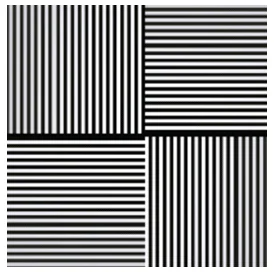
\includegraphics[width=0.47\textwidth]{Figure/Edmund/abberations-2a.png}\hfill
                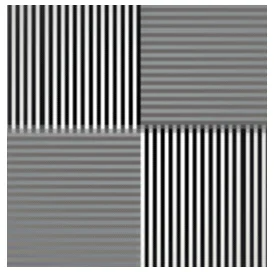
\includegraphics[width=0.47\textwidth]{Figure/Edmund/abberations-2b.png}
                \caption{左:无像散（各方向均匀清晰）\quad 右:有像散（一个方向清晰，另一个方向模糊）}
                \label{fig:edmund_astig_bars}
            \end{figure}
        \end{column}
        \hfill
        \begin{column}{.45\textwidth}
            \textbf{像散的直观表现:}
            当观察一组水平和垂直条棒时:
            \begin{itemize}
                \item 子午(切向)方向清晰 $\rightarrow$ 弧矢方向模糊
                \item 或反之
                \item \alert{两个方向无法同时聚焦}
            \end{itemize}

            \bigbreak
            \textbf{物理原因:}
            离轴光线不经过旋转对称的表面——轴上光线看到的是圆对称，离轴光线看到的是\alert{不对称的截面}。
        \end{column}
    \end{columns}
\end{frame}

\englishtitle{Off-Axis Asymmetry and Correction}
\begin{frame}{离轴不对称性与像散校正}
    \begin{columns}[T]
        \begin{column}{.50\textwidth}
            \begin{figure}
                \centering
                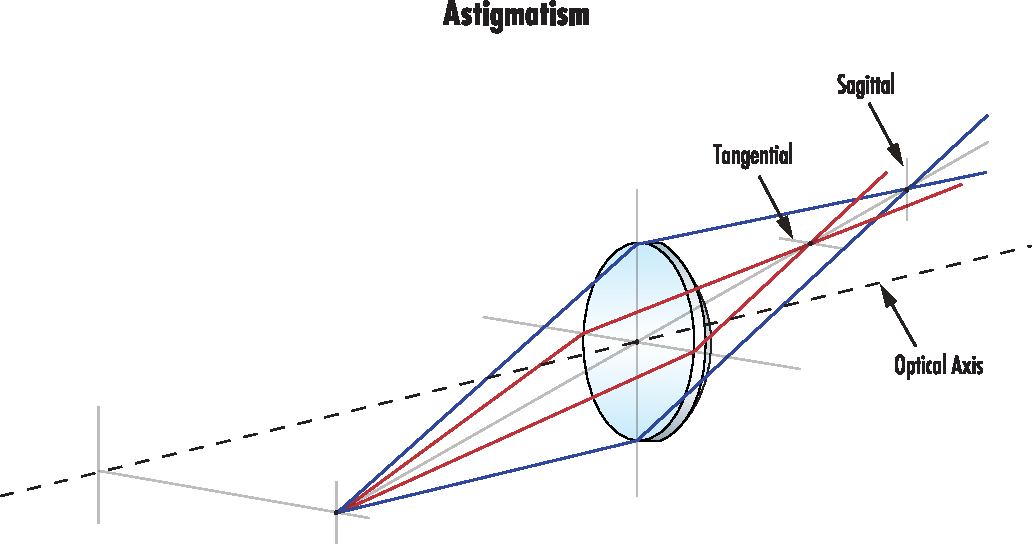
\includegraphics[width=\textwidth]{Figure/Edmund/aberrations-3v3.pdf}
                \caption{离轴不对称:子午焦点与弧矢焦点不同}
                \label{fig:edmund_off_axis}
            \end{figure}
        \end{column}
        \hfill
        \begin{column}{.50\textwidth}
            \textbf{校正策略:}
            \begin{enumerate}
                \item \alert{对称设计}:光阑两侧结构对称(如双高斯结构)
                \item \alert{低入射角}:减小离轴光线在各面上的入射角
            \end{enumerate}

            \bigbreak
            \textbf{对称设计的代价:}
            \begin{itemize}
                \item 无法使用远摄或反远摄结构
                \item 长焦镜头体积大
                \item 短焦镜头后工作距短
            \end{itemize}

            \bigbreak
            \alert{像散和彗差}在实际镜头中常共同出现，Edmund Optics 将其合并讨论。
        \end{column}
    \end{columns}
\end{frame}

\subsection{场曲与色差:像面与波长的控制}

\englishtitle{Field Curvature — The Petzval Problem}
\begin{frame}{场曲:佩兹伐和问题}
    \begin{columns}[T]
        \begin{column}{.45\textwidth}
            \begin{figure}
                \centering
                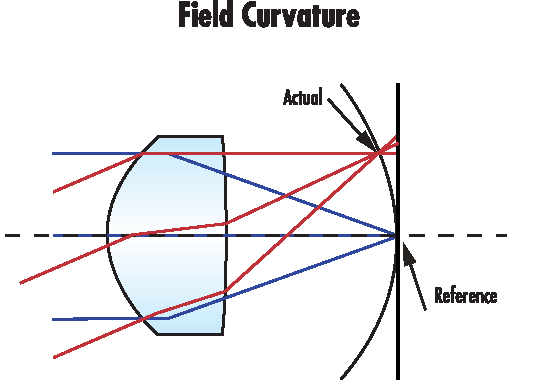
\includegraphics[width=0.9\textwidth]{Figure/Edmund/aberrations-4v2.pdf}
                \caption{场曲:最佳聚焦面是非平面的曲面}
                \label{fig:edmund_field_curv}
            \end{figure}
        \end{column}
        \hfill
        \begin{column}{.55\textwidth}
            \textbf{场曲的物理原因:}
            系统中所有透镜焦距的总和(乘以折射率)\alert{不等于零}:
            \begin{equation}
                \sum \frac{\phi_i}{n_i} \neq 0 \quad\text{(佩兹伐和)}
                \label{eq:petzval_edmund}
            \end{equation}

            若佩兹伐和为正值(成像镜头常见)，像面呈\alert{凹形弯曲}。

            \bigbreak
            \textbf{校正方法:}
            插入\alert{负光焦度校正元件}使佩兹伐和趋近于零。

            \textbf{代价:}
            镜头变长，负透镜需靠近像面，\alert{后工作距缩短}。
        \end{column}
    \end{columns}

    % \alert{机器视觉的现实:}弯曲探测器几乎不可行——必须通过光学设计校正场曲。
\end{frame}

\englishtitle{Chromatic Aberration — Wavelength-Dependent Focus}
\begin{frame}{色差:波长依赖性的焦点偏移}
    \begin{columns}[T]
        \begin{column}{.55\textwidth}
            \begin{figure}
                \centering
                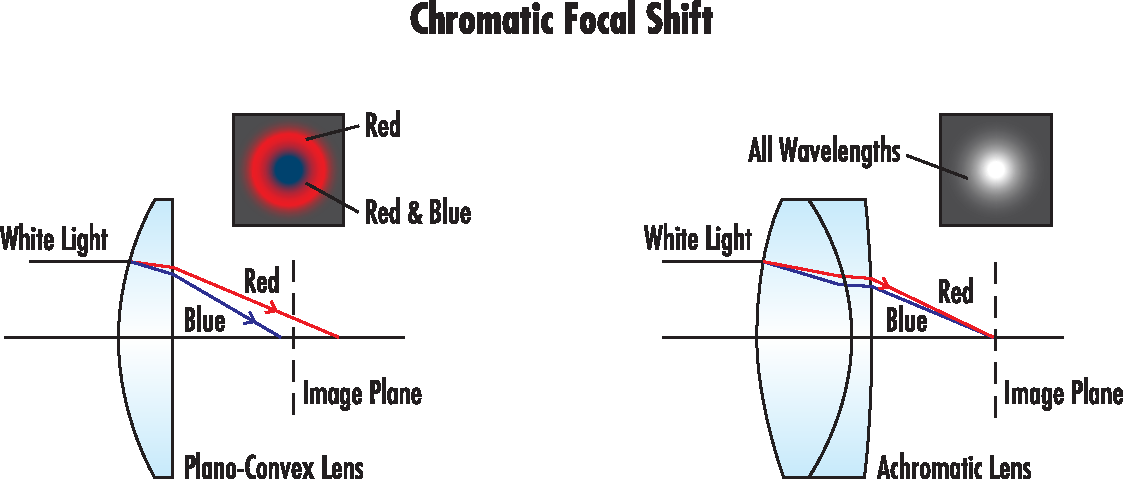
\includegraphics[width=0.95\textwidth]{Figure/Edmund/aberrations-5v2.pdf}
                \caption{单透镜 vs 消色差双胶合的光斑比较}
                \label{fig:edmund_chromatic}
            \end{figure}
        \end{column}
        \hfill
        \begin{column}{.45\textwidth}
            \textbf{色差的根源:}
            玻璃的折射率随波长变化($n(\lambda)$)，长波长光的焦距相对较长。

            \bigbreak
            \textbf{消色差原理:}
            使用\alert{正透镜 + 负透镜}组合，分别选用\alert{不同色散特性}的玻璃:
            \begin{itemize}
                \item 冕牌玻璃(高阿贝数，低色散)
                \item 火石玻璃(低阿贝数，高色散)
            \end{itemize}

            \bigbreak
            \textbf{校正的代价:}
            \begin{itemize}
                \item 镜片数量增加
                \item 消色差玻璃通常\alert{更贵、更难加工}
                \item 使用\alert{单色光源}可大幅节省成本和复杂度
            \end{itemize}
        \end{column}
    \end{columns}
\end{frame}

\englishtitle{Chromatic Focal Shift — Achromat vs Apochromat}
\begin{frame}{色焦移:消色差 vs 复消色差}
    \begin{columns}[T]
        \begin{column}{.40\textwidth}
            \begin{figure}
                \centering
                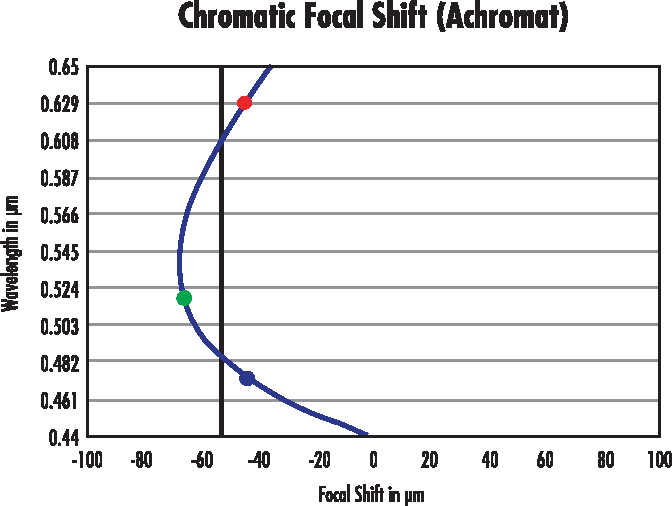
\includegraphics[width=0.92\textwidth]{Figure/Edmund/aberrations-6v2.pdf}
                \caption{\alert{消色差(Achromat)}:2个波长聚焦在同一平面}
                \label{fig:edmund_achromat}
            \end{figure}
        \end{column}
        \hfill
        \begin{column}{.40\textwidth}
            \begin{figure}
                \centering
                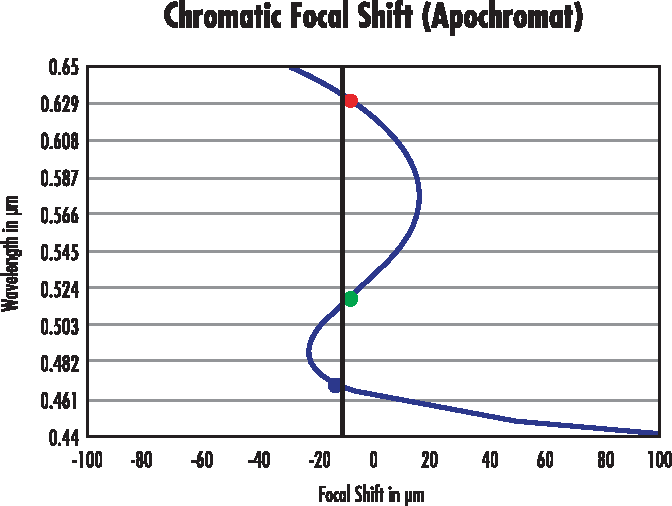
\includegraphics[width=0.92\textwidth]{Figure/Edmund/aberrations-7v2.pdf}
                \caption{\alert{复消色差(Apochromat)}:3个波长聚焦在同一平面}
                \label{fig:edmund_apochromat}
            \end{figure}
        \end{column}
    \end{columns}

    \smallbreak
    以 470nm(蓝)、520nm(绿)、630nm(红)LED 为例:
    \begin{itemize}
        \item \textbf{消色差镜}:绿光偏左，红蓝偏右——\alert{均不在最佳焦点}，但整体平衡
        \item \textbf{复消色差镜}:三色\alert{全部落在传感器平面}——图像质量最优
    \end{itemize}
\end{frame}

\englishtitle{Achromat vs Apochromat — Engineering Comparison}
\begin{frame}{消色差与复消色差的工程对比}
    \begin{table}
        \centering
        \small
        \begin{tabular}{p{2.2cm}|p{4.2cm}|p{4.2cm}}
            \toprule
            \textbf{对比维度} & \textbf{消色差 (Achromat)} & \textbf{复消色差 (Apochromat)} \\
            \midrule
            校正波长数 & \alert{2} 个波长聚焦于同一平面 & \alert{3} 个波长聚焦于同一平面 \\
            设计复杂度 & 中等，常规设计 & 高，需要特殊玻璃材料 \\
            色焦移曲线 & 与传感器平面有 2 个交点 & 与传感器平面有 3 个交点 \\
            \textbf{图像质量} & 良好(多数应用可接受) & \alert{极优}(高端检测用) \\
            适用性 & 通用性强，多种放大率 & 适用\alert{范围窄}，特定工作距 \\
            成本 & 适中 & \alert{高成本}(材料+加工) \\
            典型应用 & 一般工业相机镜头 & 显微镜物镜、高端检测 \\
            \bottomrule
        \end{tabular}
        \caption{消色差与复消色差的全面对比}
        \label{tab:achromat_vs_apochromat}
    \end{table}

    \alert{实用建议:}大多数镜头为消色差设计。对于极小像元($<2\mu$m)的传感器，消色差的残余色差可能成为问题，需考虑复消色差。
\end{frame}

\subsection{工程实践总结}

\englishtitle{Engineering Tradeoffs in Aberration Correction}
\begin{frame}{像差校正的工程权衡矩阵}
    \begin{columns}[T]
        \begin{column}{.55\textwidth}
            \textbf{所有校正方案都遵循"不可能三角":}

            \smallbreak
            \begin{block}{\centering 像质 $\uparrow$}
                \centering
                \alert{高折射率玻璃} $\nearrow$ 成本 $\uparrow$ \hspace{1.5em}
                \alert{增加镜片} $\nearrow$ 体积/重量 $\uparrow$

                \bigbreak
                \centering
                $\swarrow$ \hspace{4em} \alert{单色光源 = 低成本} \hspace{4em} $\searrow$

                \bigbreak
                {\large \textbf{成本 \hspace{3em} $\longleftrightarrow$ \hspace{3em} 体积/重量}}
            \end{block}

            \smallbreak
            \begin{center}
                \alert{$\Longrightarrow$ 工程设计的本质是找到三者之间的最优平衡点}
            \end{center}
        \end{column}
        \hfill
        \begin{column}{.48\textwidth}
            \textbf{各类像差的校正成本:}

            \begin{table}
                \centering
                \footnotesize
                \begin{tabular}{c|c|c}
                    \toprule
                    \textbf{像差} & \textbf{校正手段} & \textbf{代价} \\
                    \midrule
                    球差 & 高$n$玻璃/多片 & \$ + 体积 \\
                    像散 & 对称结构 & 体积/灵活性 \\
                    场曲 & 负光焦度元件 & 后工作距 \\
                    色差 & 消色差双胶合 & \$ + 复杂度 \\
                    复消色差 & 特殊材料 & \$\$\$ + 窄适用 \\
                    \bottomrule
                \end{tabular}
            \end{table}

            \bigbreak
            \alert{核心信息:}理解像差如何影响性能，比追求"完美校正"更重要。
        \end{column}
    \end{columns}
\end{frame}

\englishtitle{Key Messages}
\begin{frame}{像差工程要点总结}
    \begin{enumerate}
        \item \textbf{像差不是缺陷，是固有属性}——源于光的物理本质(衍射、折射、波动性)
        \item \textbf{球差}随孔径增大而恶化——缩小光圈可缓解，但衍射极限最终限制
        \item \textbf{像散}是视场依赖的——对称设计(如双高斯)是主要对策
        \item \textbf{场曲}本质是佩兹伐和问题——$\sum \phi_i/n_i \to 0$ 是目标
        \item \textbf{色差}用正负透镜+不同色散玻璃消除——消色差(2波长)vs 复消色差(3波长)
        \item \textbf{单色光照明}可大幅降低色差校正的成本和复杂度
        \item \textbf{消色差}是大多数机器视觉镜头的标准配置——足够应付常规应用
        \item \textbf{复消色差}用于高端检测——成本高、适用范围窄
        \item \alert{工程设计的本质是在像质、体积/重量和成本之间寻找最优平衡}
    \end{enumerate}
\end{frame}

\englishtitle{Integration with Transverse Aberration Analysis}
\begin{frame}{与横向像差图分析的整合视角}
    \begin{columns}[T]
        \begin{column}{.52\textwidth}
            \textbf{两种分析方法的互补关系:}

            \begin{table}
                \centering
                \small
                \begin{tabular}{p{2.5cm}|p{3cm}}
                    \toprule
                    \textbf{横向像差图分析} & \textbf{Edmund Optics 视角} \\
                    \midrule
                    精确的数学诊断 & 工程应用理解 \\
                    定量分解各像差分量 & 定性理解性能影响 \\
                    指导优化方向 & 指导设计选型 \\
                    Ray Fan / Spot & MTF / DOF / 远心度 \\
                    \bottomrule
                \end{tabular}
            \end{table}

            \bigbreak
            \textbf{整合使用:}
            \begin{enumerate}
                \item 用 Edmund 视角\alert{理解需求}:什么像差对应用最关键？
                \item 用横向像差图\alert{诊断问题}:具体是哪种像差在限制性能？
                \item 用 Zemax\alert{优化设计}:如何权衡校正方案？
            \end{enumerate}
        \end{column}
        \hfill
        \begin{column}{.48\textwidth}
            \begin{block}{从理论到实践的闭环}
                \centering
                \setlength{\fboxsep}{6pt}
                \fbox{\textbf{应用需求分析}}\\[4pt]
                \Large $\downarrow$ \\[2pt]
                \fbox{\textbf{像差诊断}}\\[4pt]
                \Large $\downarrow$ \\[2pt]
                \fbox{\textbf{Zemax 优化}}\\[4pt]
                \Large $\downarrow$ \\[2pt]
                \fbox{\textbf{性能验证}}\\[4pt]
                \small
                $\longleftarrow$ \alert{反馈迭代} $\longleftarrow$
            \end{block}
        \end{column}
    \end{columns}
\end{frame}
